\documentclass[10pt]{exam}
\usepackage[phy]{template-for-exam}
\usepackage{tikz}
\usetikzlibrary{shadings,decorations.pathmorphing,arrows.meta,shadows}

\title{Circular \#3}
\author{Rohrbach}
\date{\today}

\begin{document}
\maketitle

\begin{questions}
  
  \question
    The earth ($m_E=\SI{5.972e24}{\kilo\gram}$) is \SI{1.496e11}{\meter} away from the sun ($m_S=\SI{1.989e30}{\kilo\gram}$).

    

    \begin{parts}
      \part
        Find the force of gravity between the earth and the sun. \label{FG} 

        \vspace{2em}
        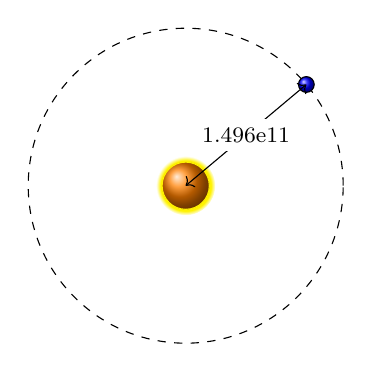
\begin{tikzpicture}[scale=0.5]
      
          \fill[
              shading=ball, 
              ball color=orange,
              circular glow={fill=yellow}, 
              draw=yellow
            ] 
            (0,0) circle (.6);
          \draw[dashed] (0,0) circle (4);
          \draw[shading=ball] 
            (40:4) coordinate (earth) circle (0.2);
          \draw[<->] (0,0) -- (earth) node[midway,fill=white] {\footnotesize \SI{1.496e11}{\meter}};
      
        \end{tikzpicture}
        \vspace{2em}

      \part
        Find the tangential velocity of the earth.  (\emph{use your answer from part \ref{FG}}) \label{vT} \vs[3]
      \part
        Find how long it takes for the earth to complete one rotation (\emph{use your answer from part \ref{vT}}) \label{T} \vs[2]
      \part
        Your answer to part \ref{T} is in seconds.  Convert it to days.  What do you notice? \vspace{5em}

    \end{parts}

  \pagebreak

  \question
    The Moon ($m_M=\SI{7.35e22}{\kilo\gram}$) is $\SI{3.9e8}{\meter}$ from the center of the Earth ($m_E=\SI{5.972e24}{\kilo\gram}$).

    

    \begin{parts}
      \part
        Find the force of gravity between the Moon and the Earth. 

        \vspace{2em}
        
        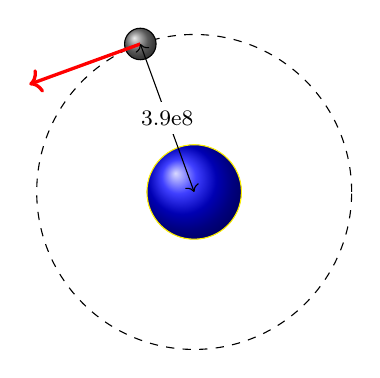
\begin{tikzpicture}
          \fill[
              shading=ball, 
              ball color=blue,
              draw=yellow
            ] 
            (0,0) circle (.6);
          \draw[dashed] (0,0) circle (2);
          \draw[
              shading=ball,
              ball color=gray
            ] 
            (110:2) coordinate (moon) circle (0.2);
          \draw[->,very thick,red] (moon) -- ++(200:1.5);
          \draw[<->] (0,0) -- (moon) node[midway,fill=white] {\footnotesize \SI{3.9e8}{\meter}};
    
        \end{tikzpicture}

        \vs
      \part
        Find the tangential velocity of the Moon.  \vs[2]

    \end{parts}



\end{questions}

\end{document}